\chapter{Deposition Procedures}
Material is sublimated from effusion cells, making molecular beams that are incident (line of sight due to high vacuum) onto heated substrate. Underneath the substrate are effusion cells which have shutters to control when material can reach substrate. The source material is contained in a crucible or as a rod is heated by either resistive heating from a refractory metal (metal that is very resistant to heat and wear) filament wound around a crucible or e-beam heating. In e-beam heating, electrons are accelerated towards source material, inducing heating when they hit. Resistive heating is suitable for lower melting pt. materials while e-beam heating is needed for high melting pt. materials (i.e. tungsten). 
\section{E-beam evaporators}
A refractory metal filament is heated by resistive heating and a high voltage is applied between the source material (either source rod or source material pellets in a crucible) and the hot filament. This draws an electron emission current from the hot filament. The emission current hits the source rod (or crucible containing  the source), making a hot tip. Once rod/crucible tip gets hot enough, the source material starts to evaporate.
\begin{figure}[H]
	\centering
	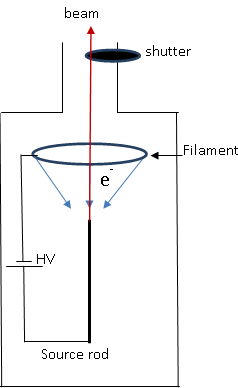
\includegraphics[width=0.5\textwidth]{e-beam_schematic.png}  %set figures width to text width
	\caption{Schematic of the e-beam evaporators}
	\label{fig:e-beam}
\end{figure}
\subsection{Currents}
It is important to keep track of three currents:\\\\
\textbf{Filament current (FIL = $\text{I}_f$):} The current flowing through a circular filament (made of refractory metal, often W) from which the electrons are coming from.  We prefer to keep it below 2.2A to lower risk of damaging the filament and extend its lifetime. Between 1.9-2.2A is a good range.  Ultimate upper limit is 2.5A, at which the filament lifetime is only 3-9 hours. Our filament is made out of Th\textsuperscript{-} doped W.\\\\
\textbf{Flux current (FLUX =  $\text{I}_{FL}$)}: Small fraction of evaporated source material will naturally be in ionized state so the current in the beam can be measured. This tells us information about the deposition rate. Current should be $>+1nA$ when material is being evaporated properly. Different materials have different degree of ionization and thus may have different flux current reading for the same deposition rate. \\\\
\textbf{Emission current (EMIS = $\text{I}_e$):} Current of electron beam going from filament to source. Will be mA order of magnitude. This current depends on FIL to heat up the filament to high enough temperature that electrons start being ejected.


\subsection{Physics of the rod positioning}
There are two controlling factors: power density and polarization, with power density being dominant. Also there is the technical limitation of maximum filament current.\\\\
\textbf{Power density:} 
If less area of the rod is being bombarded by electrons, the heating is more localized so higher temperature can be reached which results in more flux. If we move the rod too close to filament or even so it is inside the filament loop, then electrons will be bombarding a large area of the rod. This will result in a large EMIS but since heating is delocalized it will not heat up the source material enough for it to evaporate. If we did not have a maximum filament current limitation, then the best position would be as far away as possible from the filament loop so that only the tip of rod gets bombarded with electrons. However, if we position the rod too far away, then not enough of the electrons being emitted from the filament will hit the rod so we will not be able to get a high enough EMIS for flux while keeping FIL under the limit.  Therefore the objective is to find the furthest away position where can keep FIL under the upper limit while still resulting in significant FLUX. If we already have $>1nA$ FLUX and move the rod further in, while keeping EMIS the same, then FLUX will drop since have decreased power density (increased area of rod that is getting bombarded but not the number of electrons hitting it). If move rod too far in, will not be able to get any FLUX even if increase EMIS since heating is now so delocalized that can’t reach the necessary temperature for evaporation.\\\\
\textbf{Polarization:} 
Rod is polarized by the electrons hitting it which makes it harder for material to evaporate. Polarization effect is more significant on thin rods. However thin rods result in higher power density. Desired rod thickness is one that has high power density but is thick enough so that polarization is not too sever of an effect. Right now (5/2017) we use a 1.3mm diameter W rods.


\subsection{Operation Procedure}
\begin{enumerate}
\item	Turbo pump should have been running continuously overnight. 
\item	Make sure water cooling is on, the switches for all 4 MBE lines are open, and water is flowing (check the flow meters). 
\item	Turn on evaporator controller. (If are doing calibration, also move in the thickness monitor rod to the marking. Do not move it past the marking or the bevel will break). When just turn on evaporator, will see the zero values: FIL=0.12A, EMIS=0mA, voltage = 4V, Flux = ~-0.5nA (although the test sheet says +0.24nA, anyway $<1nA$ is just noise).
\item	Open gate valve (will hear loud pop sound) and turn off the ion pump: "Stop HV" on the ion pump controller. The ion pump may also be turned off a bit later, for example right before start ramping the Se evaporator.
\item	Need to fill the cryostat with liquid N2 which acts as a pump (make sure that using the in port). During filling make sure dewer hose does not touch any electrical wires. Make sure dewer has enough lquid N2 for the procedure. If run out while doing evaporation, need to turn down evaporator current and voltage and refill dewer.
\item	While filling the cryostat can start ramping the evaporaters. Once cryostat is full, immediately turn off the dewer valve but leave hose connected since will need to refill it in after about 1hr of operation. Cryostat is almost empty and needs refilling when there is almost no gas coming out the output vent at the right top of MBE chamber.
\item	On evaporator controller: first will slowly increase voltage to desired value (i.e. 800V for Sn or 2000V for W). Then start increasing current. At first the current dial controls FIL directly. Can increase FIL current to 1.5A at a moderate pace (i.e. turn slowly but don’t really have to wait for system to stabilize since it is well-behaved at this low current). When testing the evaporator for Zr (which is labeled W right now), EMIS went from 0 to 1mA when FIL reached 0.76A so that is the first point where the filament started emitting an electron beam.
\item	Once FIL reaches high enough to result in sufficient EMIS (3mA), the controller switches to feedback control and an arrow will now point to EMIS in the display. This means that now when you increase the current dial, you are increasing the set point of EMIS. The FIL current will increase until this EMIS current is reached.
\item	Once FIL $>1.5A$, need to slow down in increasing current since there is often a delay between turning the dial and system response. When see FLUX rise $>1nA$ which means that the material is being evaporated. Make sure to keep FIL preferably at $<2.2A$ in order to extend the lifetime of the filament. For W evaporation, this can be quite difficult and could require moving the rod closer to the filament after each deposition run. Every two small clicks of current dial results in about 0.1mA change in EMIS but there is sometimes up to several minute delay.
\item	If are unable to get any significant FLUX, try adjusting the rod position 0.25-1mm forward. This is done with a fine screw manipulator below the evaporator. Decreasing the mm reading means moving the rod closer to the filament. This will first result in a sudden jump in EMIS, since now more electrons hitting the rod (EMIS is measured as a circuit btw. filament and rod) larger part of rod is in the path of electron beam. Then the FIL will be lowered by the feedback loop in order to bring the EMIS down to the set point. This will allow to safely further increase the EMIS set point to try to achieve a FLUX. Higher EMIS should increase chance that will get a flux (as long as rod is not too close to filament, see below) since there are now more electrons hitting the rod.
Example: We have reached FIL = 2.2A but still have no significant FLUX. We adjust rod 1mm forward, which results in FIL to drop to 1.8A. Now we can increase EMIS set point further until FIL reaches 2.2A. If we still have no FLUX try moving rod forward again.

\end{enumerate}
According to the manual, FLUX (aka ion current) is proportional to the evaporation rate and EMIS. At a given voltage, HV and sample position FLUX is directly proportional to the flux of evaporated atoms.

Also from the manual:
When initially heat a new rod, almost all rods will melt at the tip and form a ball held by surface tension. Thus, repositioning of evaporate rod may be necessary immediately after initial heating.
Can recognize when the rod has significantly shortened in length when “at a given EMIS the high voltage has to be increased in order to obtain the same FLUX”. But in our case for W, we already are using the maximum voltage, so we will probably just see the FLUX drop when use the same EMIS. If this occurs, then need to move the rod further in. Since we do not know how much of rod has melted it is probably best to move it just 0.5mm at a time.

\section{Selenium evaporator procedures}
The selenium evaporator is made out of two parts: an effusion cell and a cracker zone. The cracker zone is a heated region near the top of the crucible (aka the hot lip). Since Se tends to evaporate in clusters, the cracker zone is used to further crack down the Se clusters which are evaporating. According to literature, temperatures for efficient cracking of Se range from 400-900C. However, due to risk of overheating the Se source (i.e. boiling), for our evaporator another group told us that 400-500C is the limit. The two zones are controlled by two separate controller. We label them EC (effusion cell) and HL (hot lip).
\begin{enumerate}
\item \textbf{Turn off the ion pump. This is essential!}.
\item Ramp both controllers slowly (15$\degree$ increments for HL and 10$\degree$ for EC) to the desired temperature. For all depositions up to May 2017, we have been using 60C for EC and between 135-155C for HL. However, we were probably not using the cracker properly and not actually cracking the Se. Also, it may be ok to use higher temperatures for EC since 100-120C seem commonly used in other groups.
\item When ready for deposition, open the Se shutter (turn 180$\degree$ from close position).
\end{enumerate}

\section{Co-deposition Overview}
For actual growth of films, the following is the general procedure:

\begin{enumerate}
	\item Assuming the substrate is already ready and on the heater stage, begin heating the sample to desired temperature with resistive heating. (\textbf{The displayed heater stage temperature is not the actual temperature of the substrate} therefore must use chart. Omicron has refused to give us a table of values for the heater stage vs. substrate relationship because their measurements are based on an average of measurements taken on many systems. They claim that the error in reading their graph chart is $<5\%$). This takes some time, so generally allow at least 1 hour to heat the sample before beginning deposition. Also the general rule we've used is to wait for the displayed heater stage temperature to be at the desired value for 30min before beginning deposition to make sure that sample has reached equilibrium with stage.
	\item Begin ramping the e-beam evaporater before Se effusion cell because the e-beam generally needs to be ramped more slowly (especially the Sn one since are using a crucible there).
	\item Turn off ion pump and ramp Se evaporater. 
	\item When everything is at desired conditions, open Se shutter. Wait 5 min. and then open the metal source shutter. (We have also opened both shutters at time and had reasonable results, so unsure that opening  Se shutter first is necessary but the idea is to establish a Se pressure in the chamber to prevent pure W or Sn from forming clusters on the sample.)
	\item When done with deposition, close both shutters and ramp everything down at reasonable pace (i.e. 10-15$\degree$ steps with Se) simultaneously. The total ramp down time takes about 10 min.
	\item Generally we want to  move the sample into STM as soon as possible after deposition to prevent it from getting contaminated by the degassing of the cryostat walls. However, it seems that the cryostat doesn't start regenerating until about 12 hours after deposition, so if necessary can move the sample up to 12 hours later.
\end{enumerate}

\section{QCM Operation}
The position of the QCM is adjusted by the bevel. The markings are:
\begin{itemize}
\item The closest to MBE sharpie mark is position for when are using the meter. This makes the QCM inside stick out from the metal shield tube so that it can measure a deposition rate and thickness.
\item The furthest from MBE sharpie mark is position for when not using the meter. This puts QCM well inside the metal shield tube so it is protected from deposited material.
\item The middle sharpie mark is bakeout position.
\end{itemize}

The reason we don’t use the QCM during actual growth is because that would wear it out too fast and it would die. To replace it, need to vent the MBE after which would need to do a bakeout! Therefore we only use QCM to calibrate (choose the proper parameters for deposition) the evaporators individually. This is how the QCM in this MBE design is intended to be used.
To use QCM:
\begin{enumerate}
\item	Move QCM to the closest to MBE sharpie mark. Connect the BNC cable connection that has a small black box along the cable. Can use an adapter to make BNC cable easier to connect. The connection is right in between the in and out water cooling ports of the QCM. Be sure water cooling is running.
\item	Turn on the thickness monitor by the switch in the back of electronics stand. Wait a few seconds and it will show some thickness and rate and frequency of QCM. 
\item	Select the material whose deposition you want to measure. There is a pre-programmed list of many materials with their properties which program needs to calculate thickness and deposition rate from QCM raw data. Also you can make your own favorites list.
\item	Press “clear” to make the thickness reading 0.
\item	Get the evaporator running at the deposition parameters but with the shutter closed, so no material is being deposited on your substrate yet. 
\item	Open the shutter on the evaporator and immediately open shutter on QCM which allows it to measure things.
\item	For some materials, the deposition slower is faster than the resolution of the rate meter (ie. $<0.1$A/s) so the rate meter will always read 0. In this case need to use the thickness meter (which is additive thickness) and divide by the running time to estimate the average deposition rate.
\end{enumerate}

\textbf{Currently, as of May 2017, the QCM is unable to detect Sn deposition}. The reason may be due to the geometry of the ports. According to Omicron, the QCM is located 20mm below the point where the beams should meet. For the E-beam evaporators, the beam is quite small, so from some ports it is possible that the beam simply doesn't hit enough of the QCM to result in a reading.

\textbf{On June 1, 2017 we switched the positions of the Sn and W evaporator and will retest the QCM}.